\chapter{Desenvolvimento}\label{cap_intro}

Usaremos as tecnologias de Java e Swing (código e telas), MongoDB (estruturar o banco de dados), Spring (comunicação com o banco de dados) e GIT (gerenciamento de versão) para criação deste sistema. Além disso, o atual escopo não prevê um controle financeiro (retorno de troco, quantidade recebida ou ainda fechamento de contas a pagar).

Outras informações pertinentes ao cadastro antes previstas como endereço, contato, desconto nas mensalidades entre outras também foram descartadas nesta versão e podem, futuramente, ser implementadas.

\section{Telas}

 A aplicação conta com duas telas onde o usuário tem a liberdade de pesquisar e cadastrar novos usuários, conforme vemos a seguir.
 
\subsection{Tela de Pesquisa}
 
 Assim que a aplicação é inicializada podemos observar (Figura 1) os filtros para a pesquisa de mensalidades dos alunos, um botão para pagamento e outro para efetuar os cadastros.
 
 \begin{figure}[H]
 	\centering
 	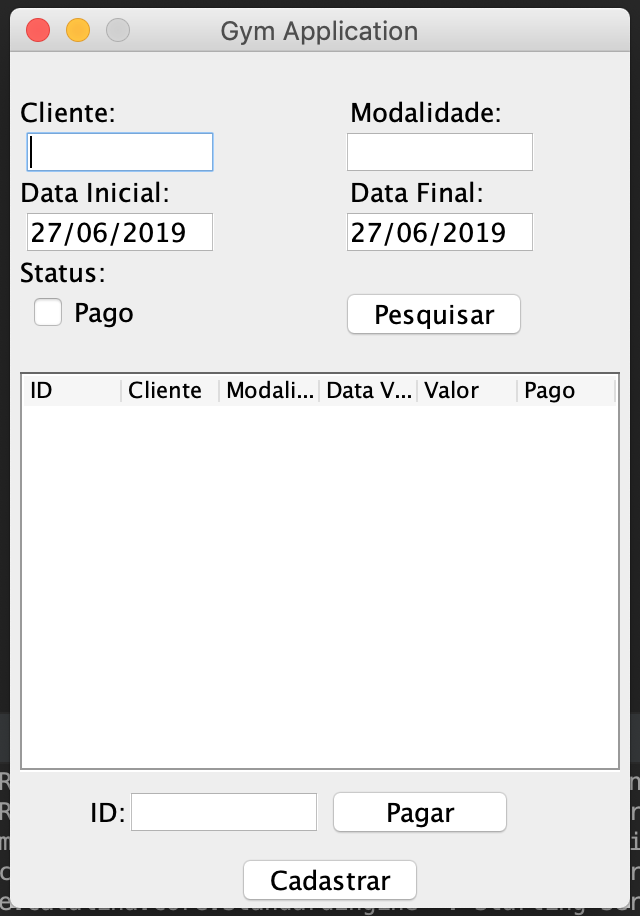
\includegraphics[width=0.5\linewidth]{images/telaBuscaVazia}
 	\caption{Tela de Pesquisa vazia}
 	Fonte: pessoal.
 	\label{fig:telaBuscaVazia}
 \end{figure}
 
 No exemplo (Figura 2) é feita uma busca utilizando todos os filtros que retorna todas as mensalidades não pagas do cliente Léo vinculadas à modalidade musculação.
 
 \begin{figure}[H]
 	\centering
 	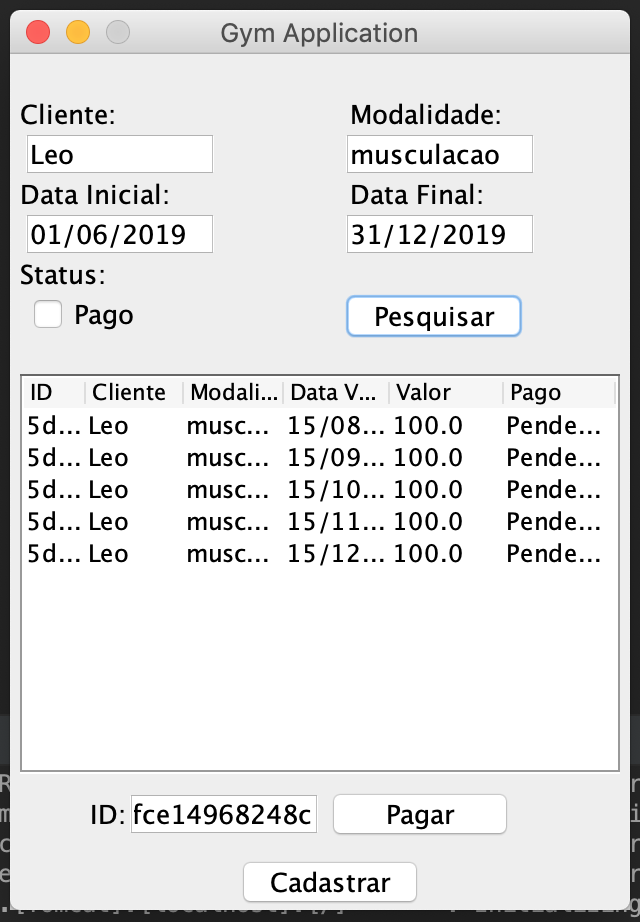
\includegraphics[width=0.5\linewidth]{images/telaBuscaPreenchida}
 	\caption{Exemplo de pesquisa na Tela de Pesquisa}
 	Fonte: pessoal.
 	\label{fig:telaBuscaPreenchida}
 \end{figure}

 Ainda é possível verificar na figura que houve o pagamento das parcelas referente aos meses 06 e 07.
 
Evidentemente, uma nova pesquisa com o filtro pago aplicado resulta na exibição das duas parcelas pagas (Figura 3).

 \begin{figure}[H]
	\centering
	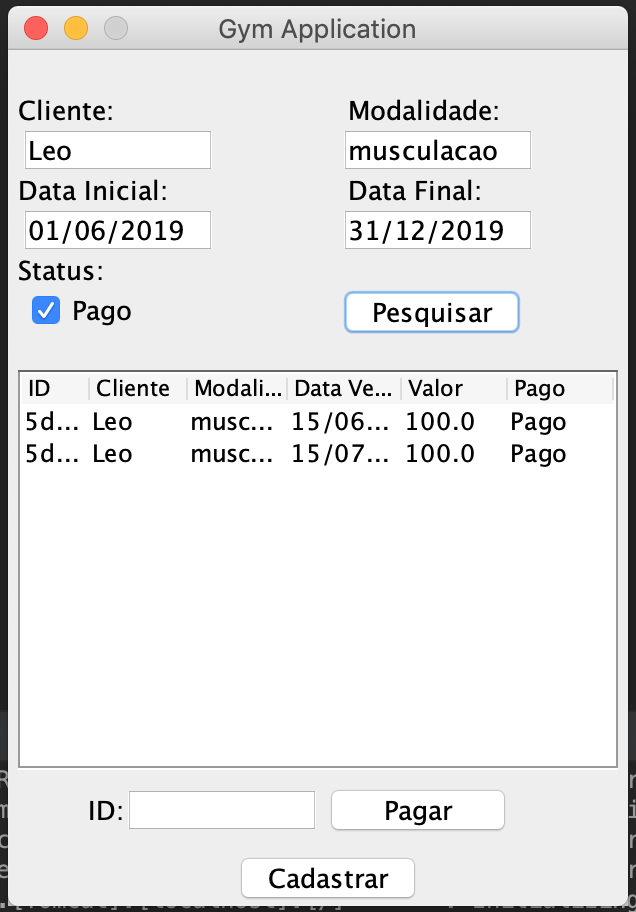
\includegraphics[width=0.5\linewidth]{images/telaBuscaPreenchidaPaga}
	\caption{Exemplo de pesquisa na Tela de Pesquisa}
	Fonte: pessoal.
	\label{fig:telaBuscaPreenchidaPaga}
\end{figure}

\subsection{Tela de Cadastro} 
 
 A Tela de Pesquisa introduz o acesso ao botão Cadastrar que possibilita o usuário inserir novos alunos, vinculando as modalidades, valores e a data de vencimento da parcela (Figura 4).
 
 \begin{figure}[H]
 	\centering
 	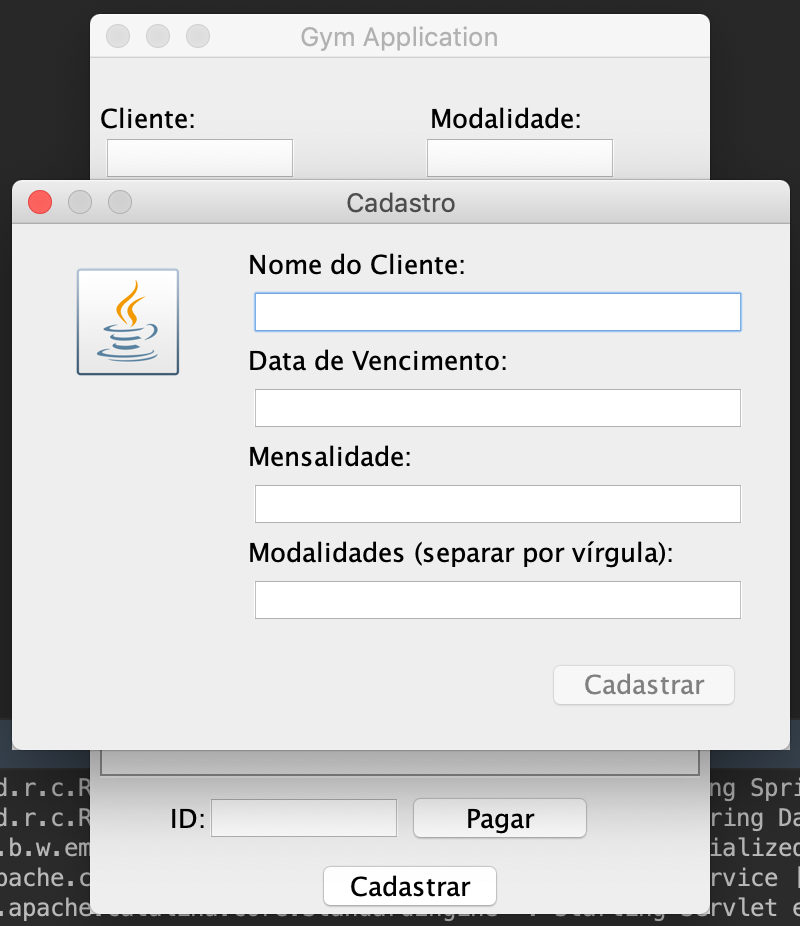
\includegraphics[width=0.5\linewidth]{images/telaCadastroVazia}
 	\caption{Tela de Cadastro vazia}
 	Fonte: pessoal.
 	\label{fig:telaCadastroVazia}
 \end{figure}
 
 Como podemos observar, os quatro campos devem ser preenchidos para que o cadastro seja efetuado.
 
 Uma vez que o preenchimento obrigatório ocorreu, é possível efetuar o cadastro (Figura 5) que poderá ser visualizado com os filtros adequados na Tela de Pesquisa.
 
 \begin{figure}[H]
 	\centering
 	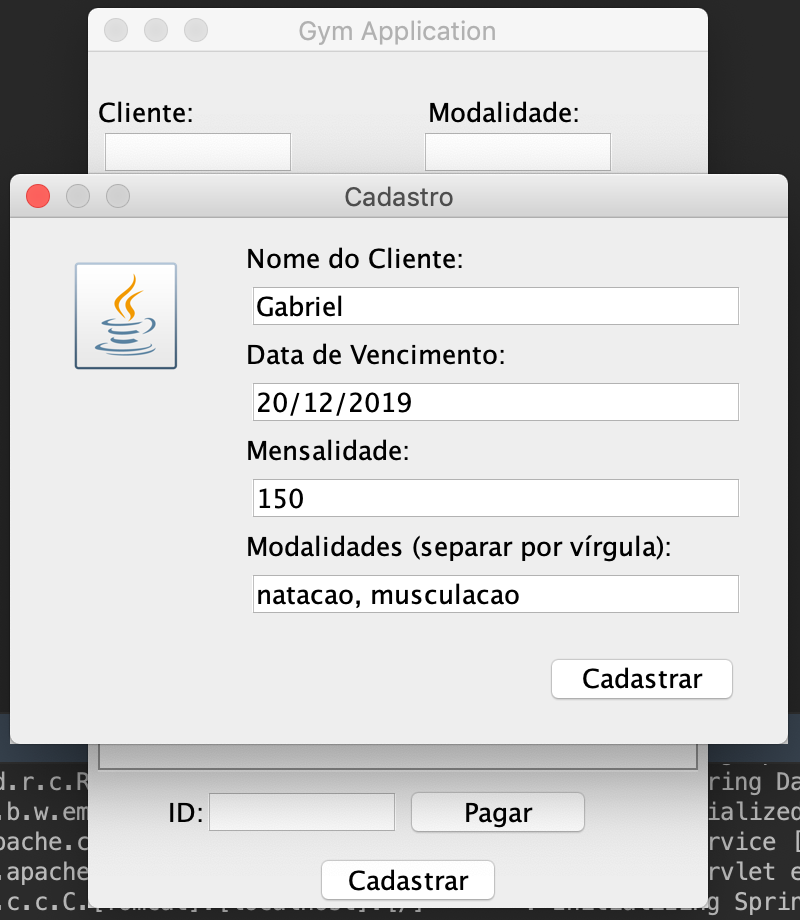
\includegraphics[width=0.5\linewidth]{images/telaCadastroPreenchida}
 	\caption{Exemplo de cadastro na Tela de Cadastro}
 	Fonte: pessoal.
 	\label{fig:telaCadastroPreenchida}
 \end{figure}
 
 Evidentemente, a busca com os filtros adequados resultam no preenchimento da tabela com os dados cadastrados (Figura 6) e possibilita o usuário a realizar as baixas necessárias.
 
 \begin{figure}[H]
 	\centering
 	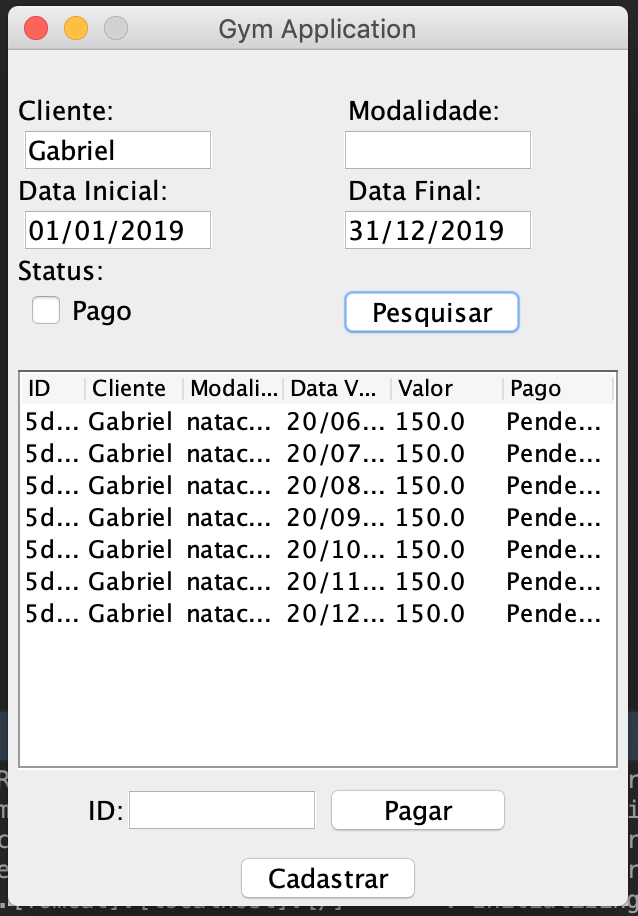
\includegraphics[width=0.5\linewidth]{images/telaCadastroBuscaAposCadastro}
 	\caption{Exemplo de pesquisa na Tela de Cadastro}
 	Fonte: pessoal.
 	\label{fig:telaCadastroBuscaAposCadastro}
 \end{figure}
 
 \section{Back-End}
 
 A construção das tabelas se dá conforme segue:

\begin{figure}[H]
	\centering
	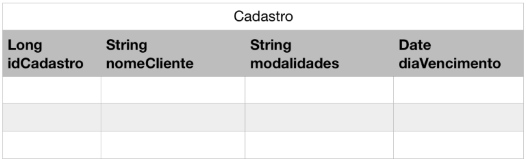
\includegraphics[width=0.7\linewidth]{images/tabelaCadastro}
	\caption{Tabela cadastro}
	Fonte: pessoal.
	\label{fig:tabelaCadastro}
\end{figure}

\begin{figure}[H]
	\centering
	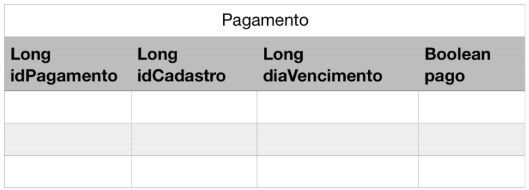
\includegraphics[width=0.7\linewidth]{images/tabelaPagamento}
	\caption{Tabela Pagamento}
	Fonte: pessoal.
	\label{fig:tabelaPagamento}
\end{figure}